%%
%% Author: Dario Chinelli
%% begin 2019-12-04
%% last mod 2022-02-02
%%

% Preamble
\documentclass[class=article, crop=false]{standalone}

% Packages
\usepackage[subpreambles=true]{standalone}
\usepackage{import}
\usepackage{graphicx}
\usepackage{amsmath}

% Document
\begin{document}

% \subsection{Metaforum}

% \subsection{Train field 7}

% \subsection{Glow experiment}

\subsection{Utrecht Centraal (Floorefield 10)}
In collaboration with ProRail - the company responsible of the train's stations in Netherlands - we had the possibility to use data from the Utrecht's train station.
The (Figure \ref{trainf10}) represents the camera's point of view of the analyzed domain in the station.
This is an interesting spot given that this square has three free sides where people could walk through.
It's also a huge corridor and an highly crossed spot, that increase the statistic.
With this domain we could study if the simulations we're doing are correct also in cases where people with different directions cross the same coordinates in the map.
In fact - as described in the following paragraphs - the representation with the 3-dimensional histogram shows us a sort of \emph{cross} X.
\begin{figure}[h]
\centering
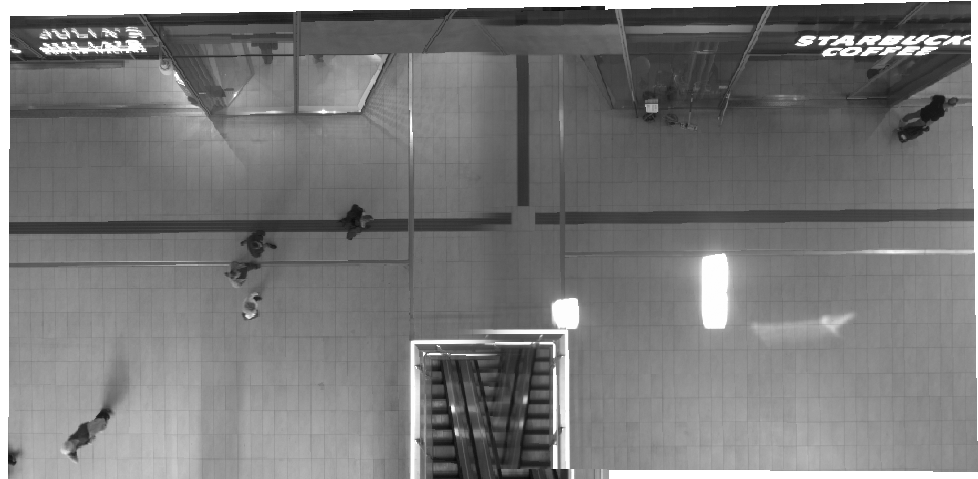
\includegraphics[width=0.4\textheight]{imgs/bg10.png}
\caption{Utrecht Centraal, cameras point of view (Floorfield 10)}
%\cite{bibliography}
\label{trainf10}
\end{figure}







\end{document}